\subsection{Translational forces from a Laboratory scale magnet (up to 180 Gauss)}
\label{sec:res_labscale-Translational}

Figure \ref{fig:fit} shows a plot of the observed unitless displacement, [tan($\alpha$)] against the magnetic field properties (B$\nabla$B) in $T^2/m$, which were determined from mapping the magnetic field. Figure \ref{fig:curve_fit_plot} is a representation of Equation \ref{eq:forFit}, it shows a linear fit with a slope of 160.3186 $\pm$ 8.2631 and intercept 0.0160 $\pm$ 0.003. Figure \ref{fig:residuals_plot}, shows the residuals for the linear fit suggesting this fit is appropiate.

\begin{figure}[htb!]
	\centering

	\subfigure[Curve fit of measured pendulum deflection vs. applied magnetic force.\label{fig:curve_fit_plot}]{
	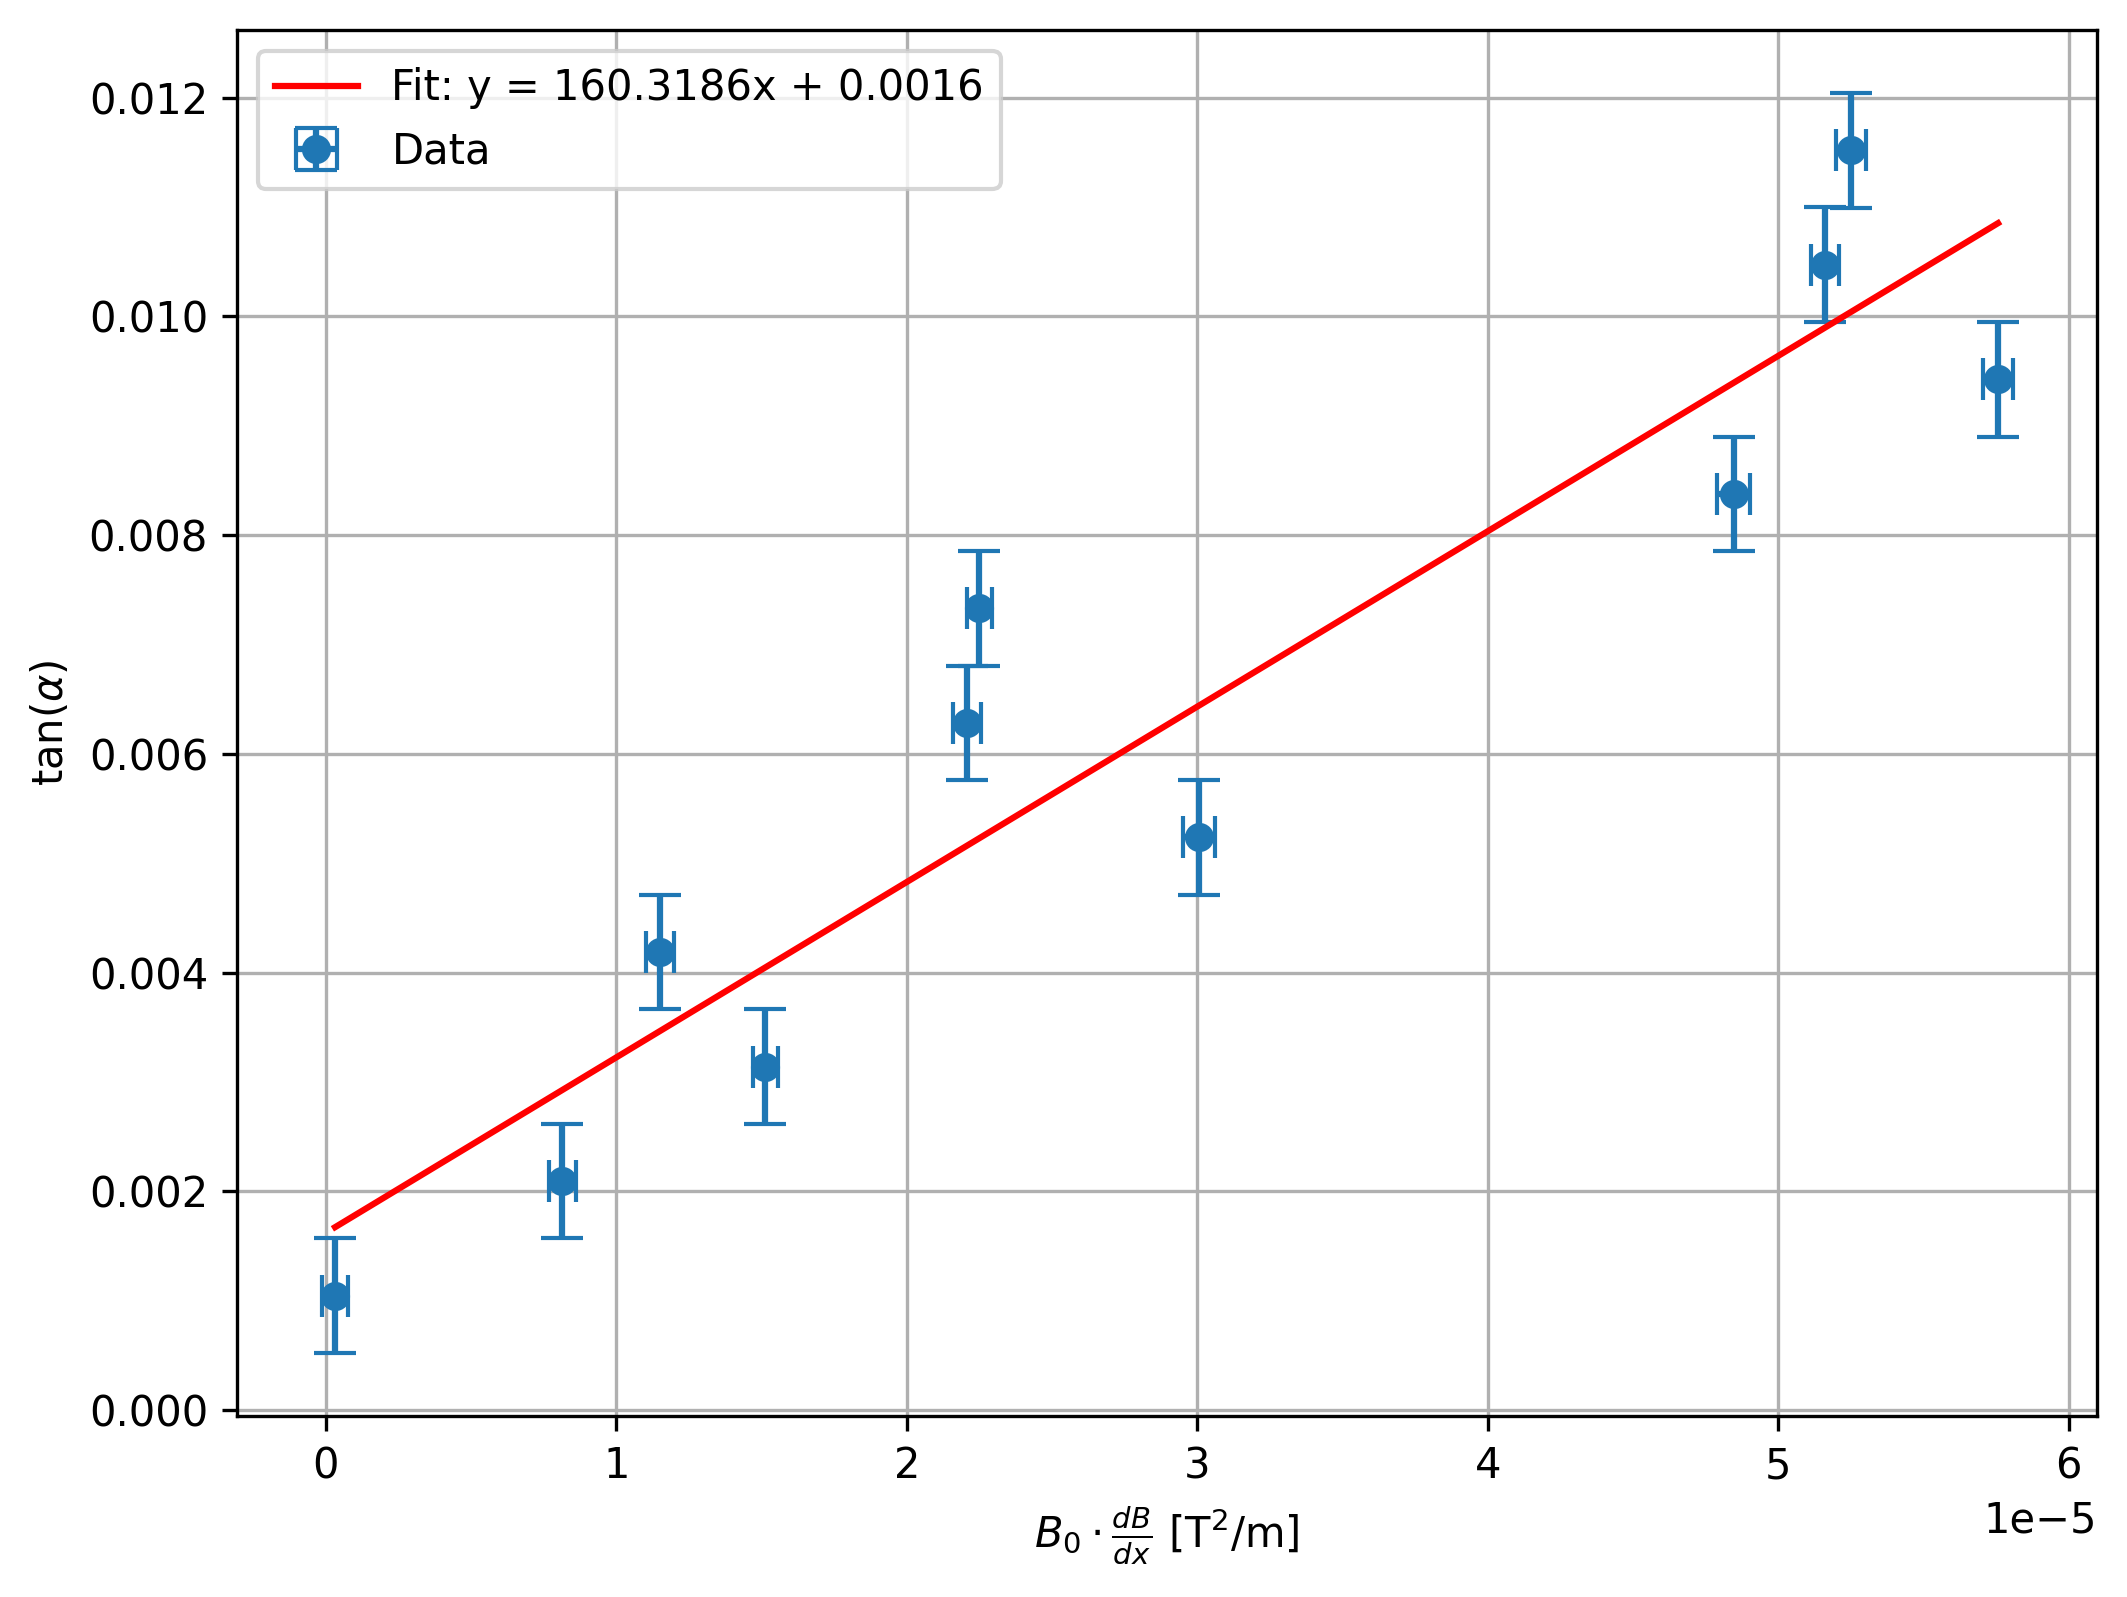
\includegraphics[width=0.9\textwidth]{Assets/curve_fit_plot.png}
	}
	\hfill
	\subfigure[Residuals from linear fit of $\tan(\alpha)$ vs. $B_0 \cdot \frac{dB_0}{dz}$. Error bars indicate propagated uncertainties.\label{fig:residuals_plot}]{
		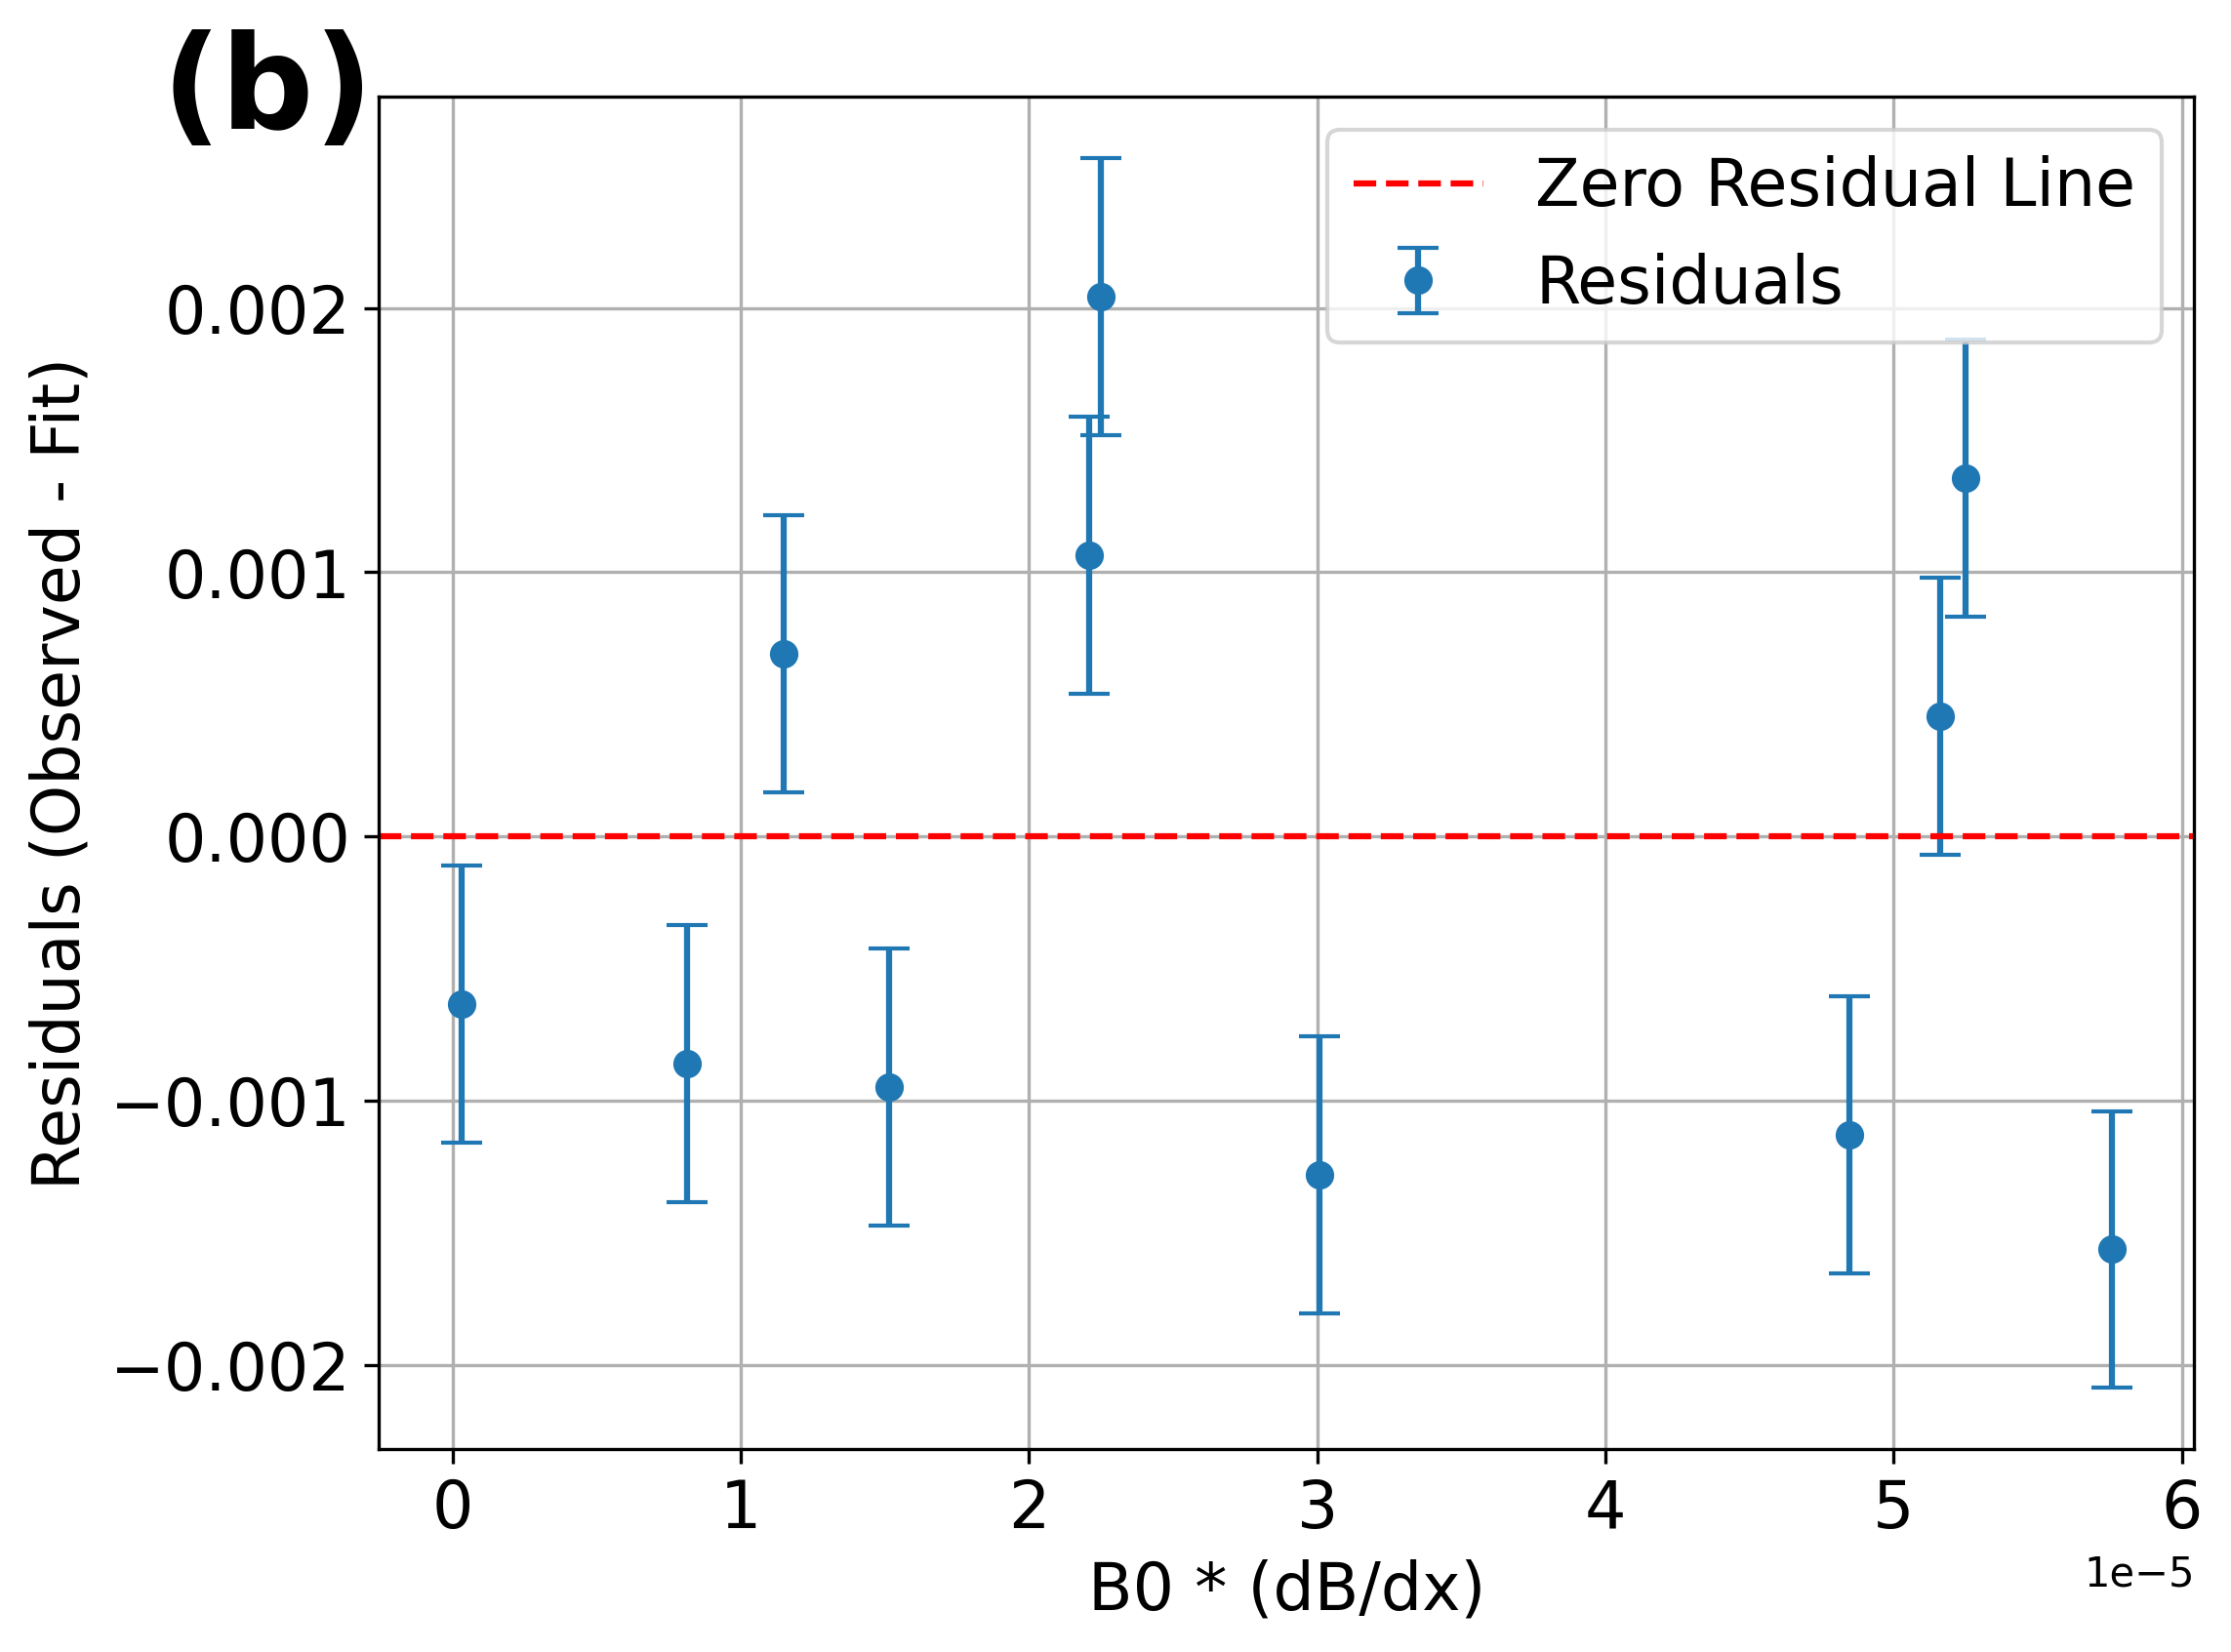
\includegraphics[width=0.9\textwidth]{Assets/Residuals_Plot.png}
	}
	\caption[Residuals and curve fit comparison]{: (a) residuals from the linearized fit, and (b) fitted curve against the measured data points.}
	\label{fig:fit}
\end{figure}

 Following Equation \ref{eq:forFit}, it can be quickly inferred that the magnetic susceptibility of the our sample is given by 
 
 \begin{equation}
 \chi = m (\mu_0 \rho g)  
 \end{equation}

\noindent where $m$ is the slope found with Figure's \ref{fig:curve_fit_plot} fit, $\mu_0$ the vacuum permittivity, $\rho$ the material's density and $g$ gravity. Sample characteristics are shown in Table \ref{tab:subjectProp}. This table shows the measured quantities, length, diameter and mass with its calculated relevant parameters (Volume, Density [$\rho$] and magnetic susceptibility [$\chi$])


\begin{table}[htb!]
	\centering
	\caption[Properties of the magnetic subject – experimental and theoretical values]{Measured and calculated characteristics of our magnetic subject depicted in Figure \ref{fig:ferrobject}}
	\begin{tabular}{lcc}
		\hline
		Property & Value & Unit \\
		\hline
		Length & $6.00 \pm 0.01$ & mm \\
		Diameter & $3.00 \pm 0.01$ & mm \\
		Mass & $0.3648 \pm 0.0001$ & g \\
		\hline
		Volume & $(4.241 \pm 0.029) \times 10^{-8}$ & m$^3$ \\
		Density & $8601 \pm 59$ & kg/m$^3$ \\
		Mass magnetic susceptibility [$\frac{\chi}{\rho}$] & $(2.01 \pm 0.05) \times 10^{-3}$ & m$^3$/kg \\
		Magnetic susceptibility (unitless) & $17.29 \pm 0.12$ & \\
		\hline
	\end{tabular}
	\label{tab:subjectProp}
\end{table}

Importantly, from Figure \ref{fig:curve_fit_plot}, tan($\alpha$) is in the range of 0.002 to 0.012. From Equation \ref{eq:deflectionAngle}, and according to ASTM 2052 \cite{astmF2052}, the force ratio threshold for MRI safety indicates 1 or, equivalently, a deflection angle of 45$^\circ$ putting our measurements way bellow that threshold for our lab simulation. In the clinic, the magnetic field is about 1.7 hundred times bigger than what we found in our lab. With samples being paramagnetic, roughly 1 million to 10 million times smaller than what we found here.


\subsection{Translational forces observed in a 3T Siemens Magnetom\textsuperscript{\texttrademark} \gls{mri} scanner}

\FloatBarrier
